\documentclass[11pt,a4paper]{article}
\usepackage[utf8]{inputenc}
\usepackage[T1]{fontenc}
\usepackage{lmodern}
\usepackage[margin=2.4cm]{geometry}
\usepackage{amsmath,amssymb}
\usepackage{graphicx}
\usepackage{booktabs}
\usepackage{xcolor}
\usepackage{hyperref}
\hypersetup{colorlinks=true,linkcolor=blue!50!black,urlcolor=blue!50!black}

\newcommand{\dd}{\mathrm{d}}
\newcommand{\kd}{k_1^{d}}

\title{Deux ressorts en série dont un endommageable :\\
solutions analytique, statique et dynamique}
\author{Dossier \texttt{ressort\_endommagement/}}
\date{\today}

\begin{document}
\maketitle

\section{Cas traité}

On considère deux ressorts (barres élastiques) en série :
\begin{center}
noeud 0 (encastré) $\;\xrightarrow{\;\text{ressort 1, } \kd(u_1)\;}\;$ noeud 1 (masse $m_1$)
$\;\xrightarrow{\;\text{ressort 2, } k_2\;}\;$ noeud 2 ($u_2$ imposé)
\end{center}
Le ressort 1 est endommageable, le ressort 2 reste élastique linéaire. Le chargement est piloté en
déplacement : on impose $u_2$ au noeud~2, croissant de $0$ à $u_2^f$. L'inconnue est le déplacement
$u_1$ du noeud intermédiaire. Le ressort 1 s'adoucit avec l'endommagement, ce qui produit un
\emph{snap-back} : la branche d'équilibre $F(u_2)$ rebrousse chemin en $u_2$, et un pilotage en
déplacement quasi-statique ne peut pas la suivre. On compare :
\begin{enumerate}
  \item la solution \textbf{analytique} (forme fermée, branche complète y compris la partie instable) ;
  \item la solution \textbf{statique} (Newton--Raphson à chaque incrément de $u_2$) ;
  \item la solution \textbf{dynamique} (masse $m_1$ au noeud 1, schéma de Newmark implicite,
        Newton--Raphson à chaque pas de temps).
\end{enumerate}
L'objet de la comparaison est en particulier la forme du résidu $R(u_1)$ que doit annuler le
Newton--Raphson, et la façon dont le terme d'inertie régularise sa non-monotonie.

\subsection{Loi d'endommagement}
L'endommagement du ressort 1 est une variable $d\in[0,1]$ fonction du déplacement maximal atteint
$\kappa = \max_{\tau\le t} u_1(\tau)$ (variable d'histoire, irréversibilité) :
\begin{equation}
  d(\kappa) = 1 - \exp\!\left(-\frac{\kappa^2}{u_c^2}\right),\qquad
  \kd(u_1) = k_1\,\bigl(1-d(\kappa)\bigr),\qquad
  F_1 = \kd\,u_1 .
\end{equation}
En charge ($u_1=\kappa$), $d'(u_1) = \dfrac{2u_1}{u_c^2}\exp(-u_1^2/u_c^2)$ ; en décharge
($u_1<\kappa$), $d$ est figé et le ressort décharge élastiquement avec la raideur sécante
$k_1(1-d)$. Pour un chargement monotone (cas analytique et statique), $\kappa=u_1$ en permanence.

\subsection{Paramètres}
Système d'unités cohérent N / mm / s, donc masse en tonne ($1\,\mathrm{t}=1000$~kg).
\begin{center}
\begin{tabular}{llr}
\toprule
Ressort 1 & $E_1 = 10\,000$~MPa, $A_1 = 20$~mm$^2$, $L_1 = 5$~mm & $k_1 = E_1A_1/L_1 = 40\,000$~N/mm\\
          & $u_c = 5$~mm & \\
Ressort 2 & $E_2 = 20\,000$~MPa, $A_2 = 30$~mm$^2$, $L_2 = 500$~mm & $k_2 = E_2A_2/L_2 = 1\,200$~N/mm\\
Masse     & $m_1 = 10$~t (noeud 1) & \\
Chargement & $u_2 : 0 \to u_2^f = 80$~mm & \\
Newton--Raphson & tolérance $|R|\le 10^{-6}$~N, 50 itérations max & \\
\bottomrule
\end{tabular}
\end{center}
Le rapport $k_1/k_2 = 33{,}3$ : le ressort 1 est très raide tant qu'il est sain, et presque tout le
déplacement imposé est absorbé par le ressort 2 ($u_1 \simeq u_2\,k_2/(k_1+k_2)$). La masse
$m_1=10$~t n'a rien de physique pour une barre de $20\,\mathrm{mm}^2\times5$~mm (masse réelle
$\rho A_1 L_1\sim 10^{-6}$~t) : c'est un paramètre numérique de régularisation, voir \S\ref{sec:dyn}.

\section{Solution analytique}
\label{sec:ana}
L'équilibre du noeud 1 s'écrit
\begin{equation}
  R(u_1;u_2) = \kd(u_1)\,u_1 - k_2\,(u_2-u_1) = u_1\bigl(\kd(u_1)+k_2\bigr) - k_2u_2 = 0 .
  \label{eq:res}
\end{equation}
Plutôt que de résoudre \eqref{eq:res} en $u_1$ à $u_2$ donné (équation transcendante à plusieurs
racines), on paramètre la branche d'équilibre par $u_1$ :
\begin{equation}
  u_2(u_1) = u_1\left(1+\frac{\kd(u_1)}{k_2}\right),\qquad
  F(u_1) = k_2\,(u_2-u_1) = \kd(u_1)\,u_1 = k_1\,u_1\,e^{-u_1^2/u_c^2}.
  \label{eq:ana}
\end{equation}
Avec $x=u_1/u_c$, la raideur tangente du ressort 1 est $\dd F/\dd u_1 = k_1 e^{-x^2}(1-2x^2)$ et la
tangente du système $k_t(u_1) = k_1e^{-x^2}(1-2x^2)+k_2$. On en déduit :
\begin{itemize}
  \item \textbf{pic de force} à $x=1/\sqrt2$ : $u_1 = u_c/\sqrt2 = 3{,}536$~mm,
        $F_{\max} = k_1 u_c e^{-1/2}/\sqrt2 = 85\,776$~N, $u_2 = 75{,}02$~mm ;
  \item \textbf{point limite} (snap-back) où $\dd u_2/\dd u_1 = k_t/k_2 = 0$ :
        $u_1 = 3{,}624$~mm, $u_2^{\lim} = 75{,}06$~mm ; au-delà, $u_2$ décroît le long de la branche
        d'équilibre jusqu'à $u_2 \simeq 13{,}3$~mm puis remonte sur la branche totalement endommagée
        ($d\to1$, $F\to0$, $u_2\simeq u_1$).
\end{itemize}
Un pilotage en déplacement quasi-statique ne peut donc pas dépasser $u_2^{\lim}$ sans sauter, à
$u_2$ fixé, de l'état $(u_1 = 3{,}62,\;F=F_{\max})$ à l'état $(u_1\simeq u_2,\;F\simeq0)$.

\paragraph{Bilan d'énergie du saut.}
Avec l'énergie libre $\Psi = \tfrac12 k_1(1-d)u_1^2 + \tfrac12 k_2(u_2-u_1)^2$ et la dissipation par
endommagement $\mathcal D = \int Y\,\dd d$, $Y=\tfrac12 k_1u_1^2$, le travail de la force le long de
la branche d'équilibre entre les deux états de même $u_2$ vérifie
$W = \int F\,\dd u_2 = \Psi_2-\Psi_1+\mathcal D_{\text{branche}}$. Le saut se faisant à $u_2$
constant ($W=0$), l'énergie libérée est $\Psi_1-\Psi_2 = \mathcal D_{\text{branche}} + |W|$.
Numériquement : $\Psi_1-\Psi_2 = 3\,217$~J, $\mathcal D_{\text{branche}} = 455$~J,
$|W| = 2\,762$~J. L'aire $|W|$ entre le saut vertical et la branche d'équilibre est donc l'énergie
libérée sous forme cinétique au saut, en excès de ce que la branche quasi-statique aurait dissipé
par endommagement. (Le script l'appelle \texttt{energie\_dissipee} pour rester proche des scripts
d'origine ; c'est cette interprétation qu'il faut retenir.)

\section{Solution statique}
\label{sec:stat}
On impose $u_2$ sur 2000 incréments uniformes et on résout \eqref{eq:res} par Newton--Raphson avec
la tangente analytique
\begin{equation}
  k_t(u_1) = \kd(u_1) + u_1\,\frac{\dd\kd}{\dd u_1} + k_2,\qquad
  u_1^{(i+1)} = u_1^{(i)} - \frac{R(u_1^{(i)})}{k_t(u_1^{(i)})},
\end{equation}
en partant de la solution de l'incrément précédent. Le résidu \eqref{eq:res} n'est pas monotone en
$u_1$ ($k_t<0$ pour $u_1\in[3{,}62\,;\,\simeq12]$~mm, minimum $k_t = -16\,650$~N/mm) : à $u_2$ donné
il peut avoir une ou trois racines (figure~\ref{fig:res}, gauche).

\paragraph{Traitement du saut.}
Pour $u_2 > u_2^{\lim}$ il n'y a plus de racine au voisinage de l'itéré précédent : le
Newton--Raphson cycle sans converger (dans les scripts d'origine, ce cas n'était pas détecté et une
valeur non convergée était stockée). Le solveur teste maintenant la convergence et, en cas d'échec,
relance le Newton--Raphson depuis la branche totalement endommagée ($u_1^{(0)}=u_2$) : le saut a
lieu au premier incrément après le point limite ($u_2 = 75{,}08$~mm), conformément à la solution
analytique. Hors saut, 4 itérations suffisent.

\section{Solution dynamique}
\label{sec:dyn}
On ajoute une masse $m_1$ au noeud 1 ; le noeud 2 reste piloté en déplacement par une rampe
$u_2(t)=v_2\,t$ jusqu'à $u_2^f$, puis maintenu à $u_2^f$ pendant $n_{\text{hold}}$ pas pour laisser le
saut se terminer. L'équation du mouvement du noeud 1 (sans amortissement) est
\begin{equation}
  m_1\ddot u_1 + \kd(u_1)\,u_1 - k_2\,(u_2(t)-u_1) = 0 .
\end{equation}

\paragraph{Schéma de Newmark.}
Newmark implicite, $\beta=\tfrac14$, $\gamma=\tfrac12$ (moyenne des accélérations,
inconditionnellement stable, sans amortissement numérique), sous forme prédicteur--correcteur :
\begin{align}
  \tilde u &= u_n + \Delta t\,v_n + \tfrac{\Delta t^2}{2}(1-2\beta)\,a_n, &
  \tilde v &= v_n + (1-\gamma)\Delta t\,a_n,\\
  a_{n+1} &= c_1\,(u_{n+1}-\tilde u),\quad c_1 = \frac{1}{\beta\Delta t^2}, &
  v_{n+1} &= \tilde v + \gamma\Delta t\,a_{n+1}.
\end{align}
Le résidu à annuler au pas $n+1$ et sa tangente sont ceux du cas statique augmentés du terme
d'inertie :
\begin{equation}
  R_{\text{dyn}}(u_1) = m_1c_1\,(u_1-\tilde u) + R(u_1;u_2^{n+1}),\qquad
  k_t^{\text{dyn}}(u_1) = m_1c_1 + k_t(u_1).
  \label{eq:resdyn}
\end{equation}
Le Newton--Raphson est initialisé par le prédicteur $\tilde u$. La variable d'histoire $\kappa$ est
figée pendant les itérations d'un pas et mise à jour après convergence.

\paragraph{Choix du pas de temps : régularisation inertielle.}
D'après \eqref{eq:resdyn}, l'inertie ajoute à la tangente la constante $m_1c_1 = m_1/(\beta\Delta t^2)$.
Si $m_1c_1 > -\min k_t = 16\,650$~N/mm, le résidu dynamique est strictement croissant en $u_1$ : une
seule racine, Newton--Raphson sans ambiguïté, plus de saut brutal au point limite. Avec la pulsation
propre du système sain $\omega_0=\sqrt{(k_1+k_2)/m_1} = 64{,}2$~rad/s ($T_0 = 97{,}9$~ms) et
$\Delta t = T_0/N$, le rapport inertie/raideur vaut
\begin{equation}
  \frac{m_1c_1}{k_1+k_2} = \frac{N^2}{4\pi^2\beta} = \frac{N^2}{\pi^2}\quad(\beta=\tfrac14).
\end{equation}
Un pas fin ($N=40$, choix initial) donne un rapport $\simeq160$ : le résidu dynamique est une droite
quasi parfaite et la comparaison avec le statique n'a plus d'intérêt. On retient $N=5$,
soit $\Delta t = 19{,}6$~ms, $m_1c_1 = 104\,360$~N/mm, rapport $2{,}5$ : assez pour régulariser
(tangente dynamique minimale $+87\,700$~N/mm) sans écraser la contribution du ressort endommagé. La
rampe dure 150 pas ($2{,}94$~s, soit 30 périodes propres : chargement lent devant la dynamique du
système), suivie de 100 pas de maintien. Le Newton--Raphson converge en 3 itérations au plus.

\paragraph{Résultats.}
La solution dynamique suit la branche d'équilibre analytique au-delà du point limite ($u_2$ jusqu'à
$\simeq78$~mm avant que $F$ ne décroche, figure~\ref{fig:fu}), puis le noeud 1 « saute » vers la
branche endommagée pendant le maintien. L'énergie libérée (\S\ref{sec:ana}) n'ayant aucun mécanisme
de dissipation (pas d'amortissement, ressort 1 déjà totalement endommagé), la masse oscille ensuite
librement sur le ressort 2 autour de $u_1 = u_2^f$ avec la période $2\pi\sqrt{m_1/k_2} = 0{,}574$~s
et une amplitude $\simeq73$~mm (figure~\ref{fig:temps}) ; $F_2$ devient alors alternativement
négative (ressort 2 comprimé). Grâce à l'irréversibilité ($\kappa$), l'endommagement reste $d=1$
pendant ces oscillations ; avec la loi réversible $d=d(u_1)$ des scripts d'origine, $d$ redescendait
à $0{,}66$ au point bas ($u_1\simeq5$~mm) et le ressort 1 « guérissait », ce qui est non physique.

\section{Figures}
\begin{figure}[h]\centering
  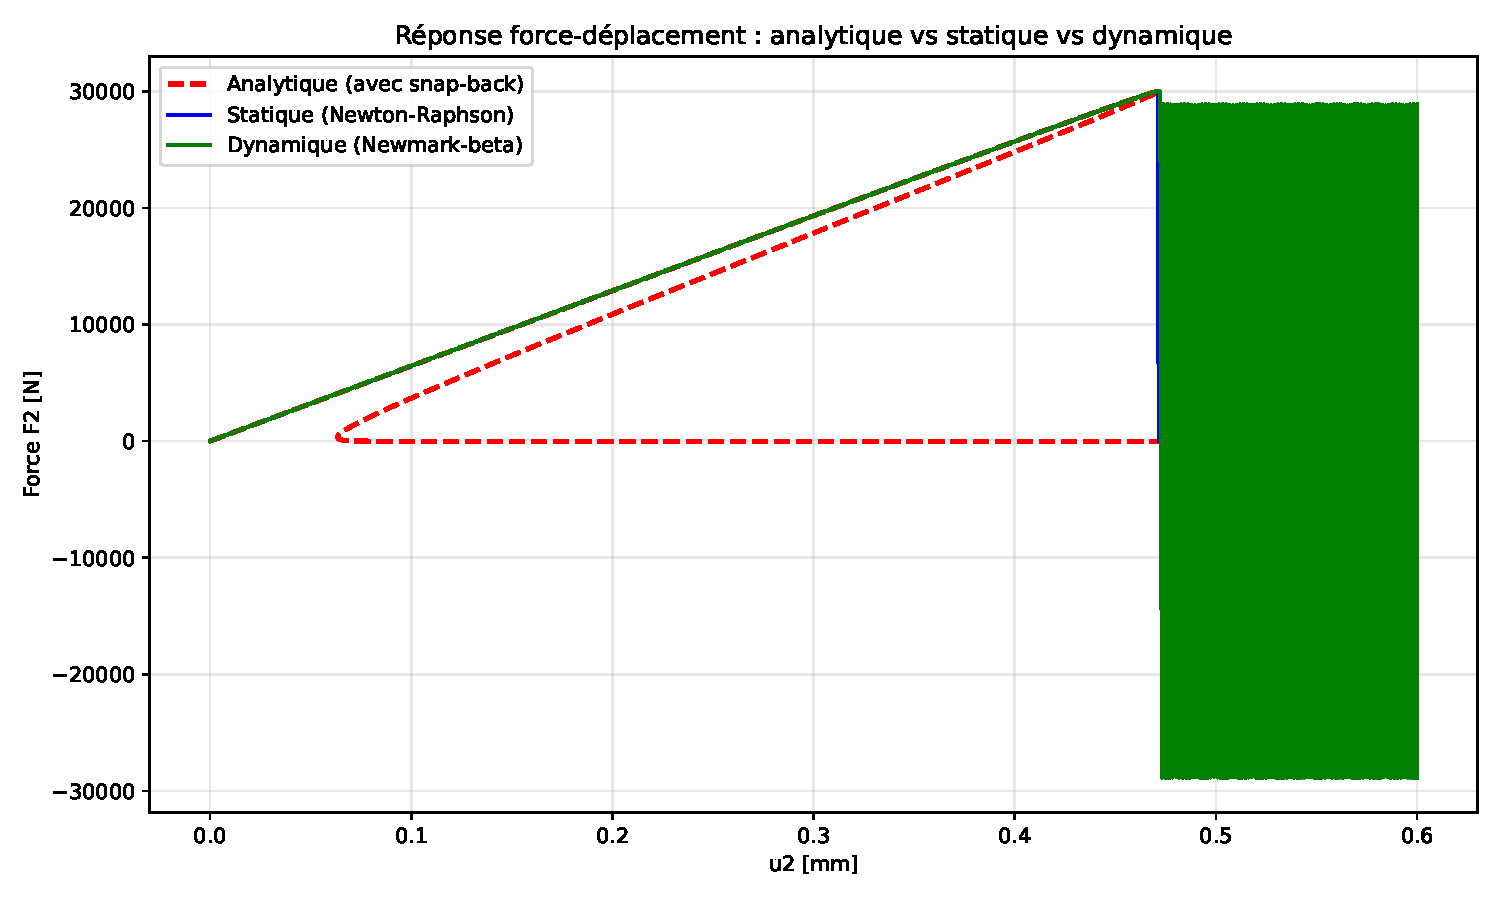
\includegraphics[width=.85\textwidth]{figures/force_deplacement.pdf}
  \caption{Réponse force--déplacement $F_2(u_2)$ : analytique (branche complète avec snap-back),
  statique (saut au point limite) et dynamique (dépasse le point limite puis saute et oscille).}
  \label{fig:fu}
\end{figure}
\begin{figure}[h]\centering
  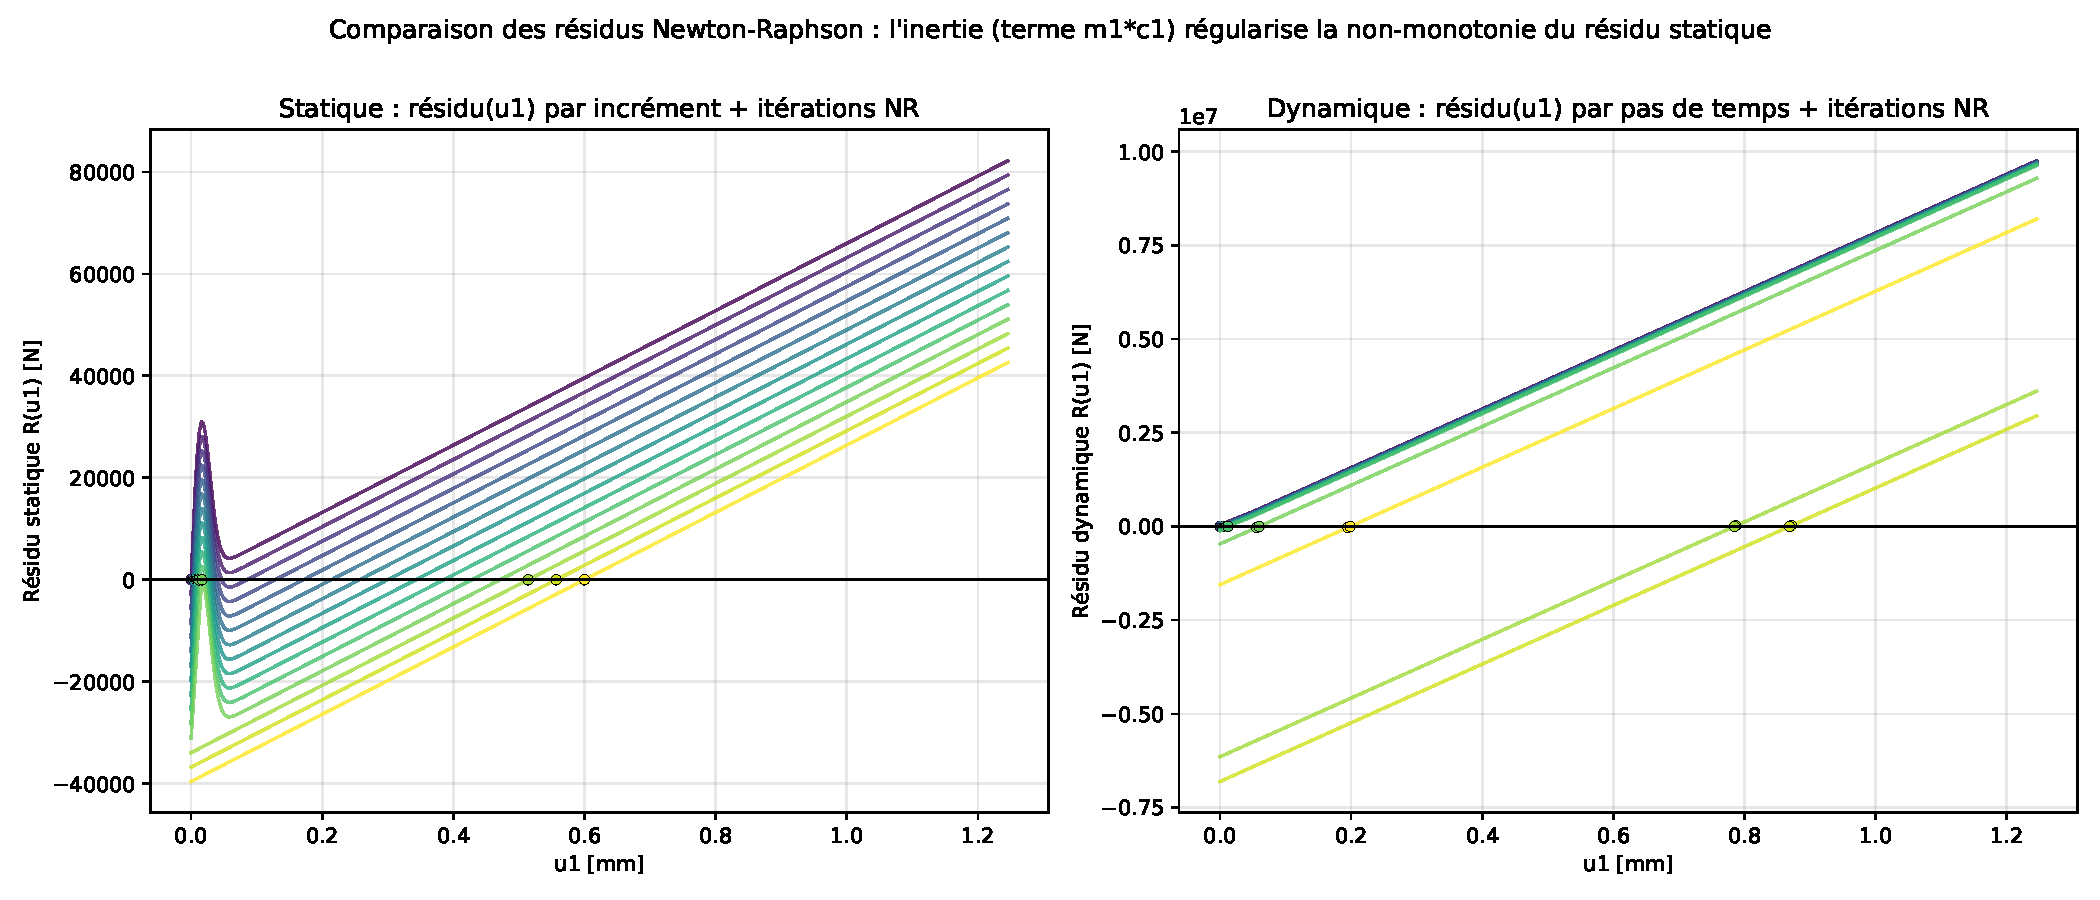
\includegraphics[width=\textwidth]{figures/residus_statique_dynamique.pdf}
  \caption{Résidu $R(u_1)$ à annuler par le Newton--Raphson, une courbe par incrément (couleur du
  violet, début de chargement, au jaune, fin) avec les itérés en points. Gauche : statique, résidu
  non monotone (bosse due à l'adoucissement du ressort 1), jusqu'à trois racines. Droite : dynamique,
  le terme $m_1c_1(u_1-\tilde u)$ rend le résidu strictement croissant ; les courbes se décalent
  verticalement avec $\tilde u$, qui porte l'histoire cinématique.}
  \label{fig:res}
\end{figure}
\begin{figure}[h]\centering
  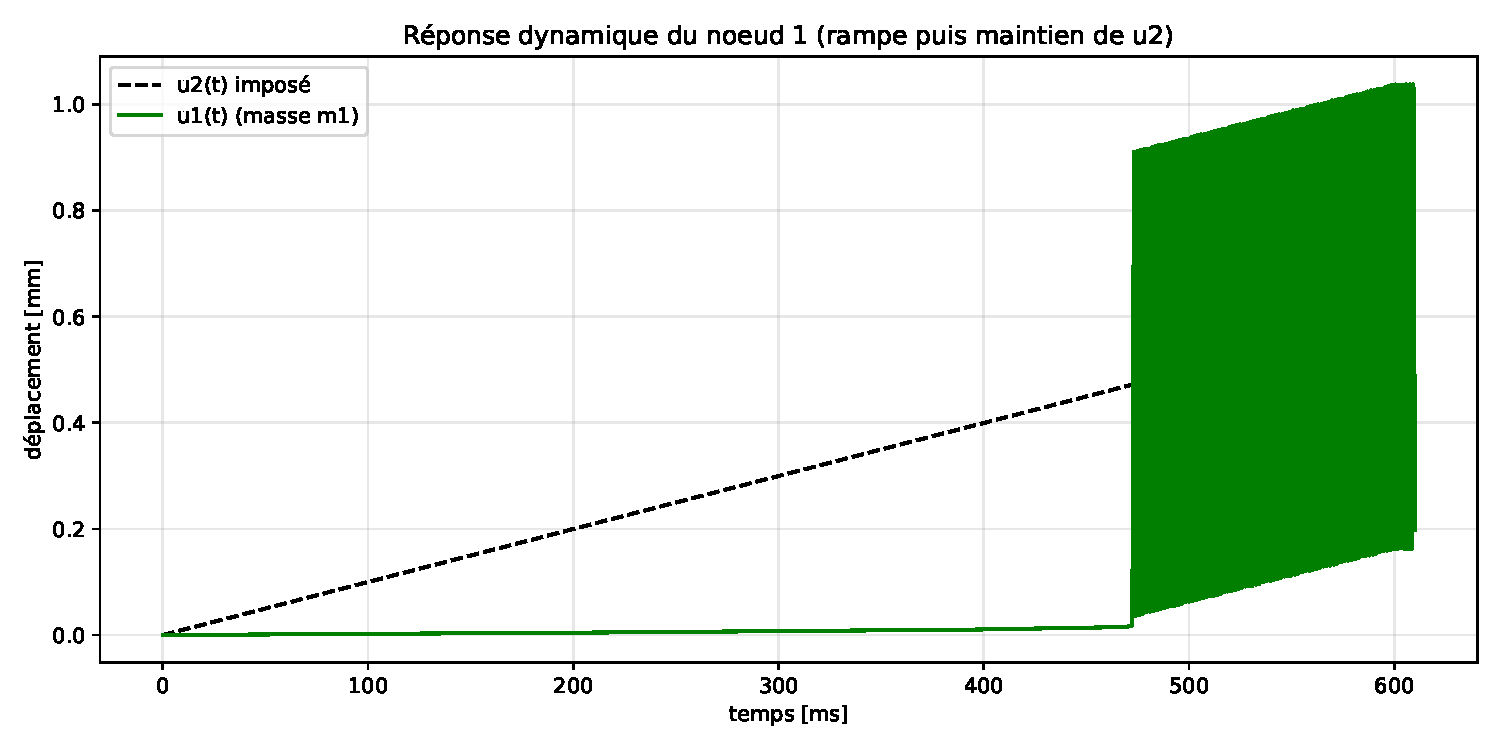
\includegraphics[width=.85\textwidth]{figures/reponse_temporelle.pdf}
  \caption{Réponse temporelle dynamique : rampe de $u_2$ puis maintien ; saut du noeud 1 et
  oscillation libre non amortie sur le ressort 2.}
  \label{fig:temps}
\end{figure}

\clearpage
\section{Organisation des scripts et vérifications}
\begin{center}
\begin{tabular}{ll}
\toprule
\texttt{modele.py} & paramètres, loi d'endommagement avec $\kappa$, résidu/tangente statiques, Newton--Raphson\\
\texttt{solution\_analytique.py} & branche \eqref{eq:ana}, pic, bilan d'énergie\\
\texttt{solution\_statique.py} & incréments de $u_2$, Newton--Raphson, relance au saut, historique des itérés\\
\texttt{solution\_dynamique.py} & Newmark prédicteur--correcteur, rampe + maintien, historique des itérés\\
\texttt{comparaison.py} & assemble les trois solutions, figures (\texttt{--save} les écrit dans \texttt{figures/})\\
\bottomrule
\end{tabular}
\end{center}
Points vérifiés : pic et point limite numériques conformes aux valeurs analytiques ; identité
$\Psi_1-\Psi_2 = \mathcal D_{\text{branche}}+|W|$ satisfaite ; convergence du Newton--Raphson à
chaque incrément/pas (tolérance $10^{-6}$~N, une tolérance de $10^{-9}$~N était sous le bruit
d'arrondi des termes d'inertie $\sim10^7$~N) ; positivité de la tangente dynamique ; période des
oscillations libres ; conservation de $d=1$ après le saut.

\paragraph{Limites et prolongements.}
Masse non physique (paramètre de régularisation) ; absence d'amortissement, d'où des oscillations
perpétuelles après le saut (un amortissement $c\,\dot u_1$ ou un Newmark dissipatif $\gamma>\tfrac12$
les ferait décroître) ; le ressort 2 est supposé sans masse ; la relance au saut statique suppose
que l'autre branche stable est la branche totalement endommagée, ce qui est le cas ici.

\end{document}
